\chapter{Optimization}

General set up of the section:
\begin{equation*}
    \begin{split}
        f: & \quad u\to\bbR, u\subseteq\bbR^n\\
        & \quad (x_1,\ldots,x_n)\to f(x_1,\ldots,x_n)
    \end{split}
\end{equation*}
\textbf{Motivation:} we are going to explore tools to compute maxima and minima of $f$.
\ex[]{$f: \bbR\to\bbR$}{
    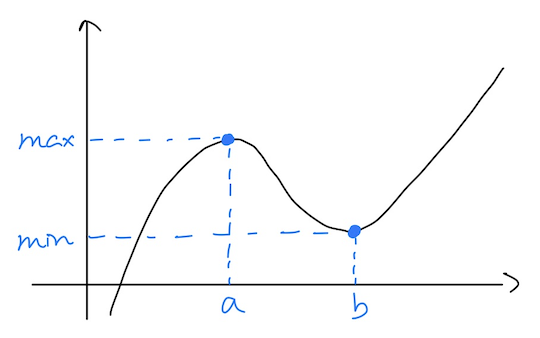
\includegraphics[scale=0.5]{Images/20.png}
}
\ex[]{$f: \bbR^2\to\bbR$}{
    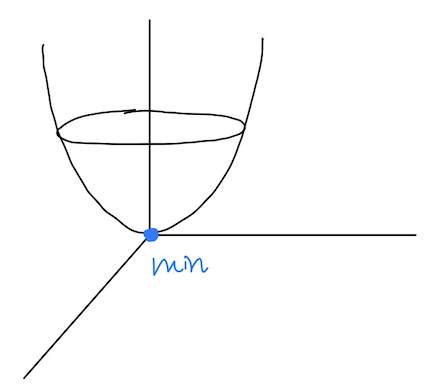
\includegraphics[scale=0.5]{Images/21.png}
}
Previously,
\begin{equation*}
    \begin{split}
        f: & \quad\bbR\to\bbR\\
        & \quad x\to x^3-x
    \end{split}
\end{equation*}
\begin{itemize}
    \item Find the domain: $D_f = \bbR$
    \item $f'(x) = 3x^2-1$
    \item Zeros of the first derivative: $f'(x)=0\Leftrightarrow x=\pm\frac{1}{\sqrt{3}} \to$ critical points
    \item Sign of $f'$ defines the monotony of $f$: $f'<0\to f$ is decreasing; $f'>0\to f$ is increasing
    \item $x=\frac{1}{\sqrt{3}}\to$ minimizer; $f(\frac{1}{\sqrt{3}})=-\frac{2\sqrt{3}}{3}\to$ minimum
    \item $x=-\frac{1}{\sqrt{3}}\to$ maximizer; $f(-\frac{1}{\sqrt{3}})=\frac{2\sqrt{3}}{3}\to$ maximum
\end{itemize}
\begin{center}
    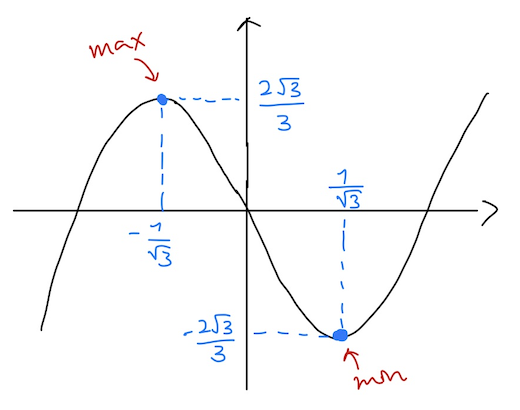
\includegraphics[scale=0.5]{Images/22.png}
\end{center}

If $f: u\to\bbR$ is a smooth map, it is not necessarily true that $f$ has a maximum or minimum.
However, if $f: K\to\bbR, K\subseteq\bbR^n$ where $K$ is compact, then $f$ has a maximum and minimum (\textbf{Weierstrass theorem}).

\section{Formal definition}


%\dfn{Definition Topic}{Definition Statement}
%\thm{Theorem Name}{Theorem Statement}
%\cor[cori]{Corollary Name}{Corollary Statement}
%\lem{Lemma Name}{Lemma Statement}
%\clm{Claim Name}{Claim Statement}
%\ex{Example Name}{Example explained}
%\opn{Open Question Name}{Question Statement}
%\pr{Question Name}{Question Statement}
%\nt{Special Note}
%\wc{Wrong Concept topic}{Explanation}
%\proof{Proof Idea}{}